\begin{frame}
\frametitle{Espace d'approximation / Points de faces}
\vfill
\begin{columns}[c]
\column{.5\textwidth}
\begin{itemize}
\item $(\Deg + 1)^2$ points et poids d'intégration de Gauss-Legendre par face :
\begin{align*}
&(\GLN{f,i})_{i \ge 0} \subset \QuadRef_f , \\
&(\GLW{f,i})_{i \ge 0} \subset \EnsR^{\star +} \ ;
\end{align*}
\item Projetés orthogonaux sur les faces des points volumiques : $i = \pi(f,j)$ ;
\item Formule de quadrature surfacique :
\begin{align*}
\int_{\QuadRef_f} \psi (\xref) d\xref \approx
	\sum_{i} \GLW{f,i} \psi (\GLN{f,i}) .
\end{align*}
\end{itemize}
\column{.5\textwidth}
\begin{figure}
\centering
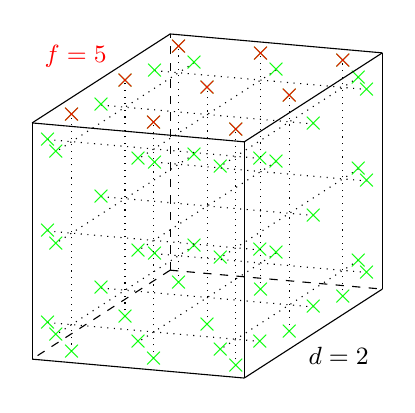
\begin{tikzpicture}[scale=3,rotate around x=270,rotate around z=258]
	% cube arriere
	\draw [dashed] (0,0,0) -- (1,0,0);
	\draw [dashed] (0,0,0) -- (0,1,0);
	\draw [dashed] (0,0,0) -- (0,0,1);

	\draw (0.7,1.25) node {\small$d=2$};
\onslide<2>{
	\draw (0.3,-0.25,1) node {\textcolor{red}{\small$f=5$}};
}

	% gauss legendre: 0.1127, 0.5, 0.8873
	\def \pgs {0.1127,0.5,0.8873}
	\def \c {0,1}

	% points surface et lignes pointilées direction x
	\foreach \y in \pgs
	\foreach \z in \pgs {
		\draw [dotted] (0,\y,\z) -- (1,\y,\z);
		\foreach \x in \c {
			\draw (\x,\y,\z) node[green] {$\bm{\times}$};
		}
	}
	% points surface et lignes pointilées direction y
	\foreach \x in \pgs
	\foreach \z in \pgs {
		\draw [dotted] (\x,0,\z) -- (\x,1,\z);
		\foreach \y in \c {
			\draw (\x,\y,\z) node[green] {$\bm{\times}$};
		}
	}
	% points surface et lignes pointilées direction z
	\foreach \x in \pgs
	\foreach \y in \pgs {
		\draw [dotted] (\x,\y,0) -- (\x,\y,1);
		\draw (\x,\y,0) node[green] {$\bm{\times}$};
\onslide<1>{
		\draw (\x,\y,1) node[green] {$\bm{\times}$};
}
\onslide<2>{
		\draw (\x,\y,1) node[red] {$\bm{\times}$};
}
	}

	% cube avant
	\draw [-] (1,1,0) -- (1,0,0);
	\draw [-] (0,1,1) -- (0,1,0);
	\draw [-] (1,0,1) -- (0,0,1);

	\draw [-] (1,1,0) -- (0,1,0);
	\draw [-] (0,1,1) -- (0,0,1);
	\draw [-] (1,0,1) -- (1,0,0);

	\draw [-] (1,1,0) -- (1,1,1);
	\draw [-] (0,1,1) -- (1,1,1);
	\draw [-] (1,0,1) -- (1,1,1);
\end{tikzpicture}
\end{figure}
\end{columns}
\vfill
\end{frame}

